\documentclass[xcolor={dvipsnames}]{beamer}

% \documentclass[handout,xcolor={dvipsnames}]{beamer}
% \usepackage{pgfpages}
% \pgfpagesuselayout{2 on 1}[a4paper,border shrink=1cm]

\usepackage{BeamerColor}
\usepackage{appendixnumberbeamer}
\usepackage{geometry}
\usepackage{tikz}
\usepackage{listings}
\usepackage{fvextra}
\usepackage{hyperref}
\renewcommand\appendixname{Appendix}
\usetikzlibrary{decorations.pathreplacing,calc,shapes,positioning,tikzmark,arrows,arrows.meta}

\usetheme[secheader]{Madrid}
% \usecolortheme{beaver}
\usecolortheme[named=SteelBlue]{structure}
\graphicspath{{./img/}}
\lstset{
    language=C++,
    columns=flexible,
    basicstyle=\scriptsize\ttfamily\color{Gray},
    keywordstyle=\bfseries\color{Blue},
    keywordstyle={[2]\bfseries\color{BlueViolet}},
    stringstyle=\color{Red},
    commentstyle=\color{Green},
    identifierstyle=\color{Black},
    numbers=none,
    captionpos=b,
    breaklines=true,
    breakatwhitespace=true,
    showstringspaces=false,
    tabsize=4,
    morecomment=[l][\color{Sepia}]{\#}
}

\title{Debugging}
\author{\href{mailto:hadi.safari@ut.ac.ir?subject=[AP\%20S98]\%20}{Hadi Safari}}
\institute[University of Tehran]{
    
\includegraphics[width=10ex]{ut}\\
    University of Tehran
}
\logo{
\includegraphics[width=10ex]{ut}}
\date[Advanced Programming (S98)]{
    Advanced Programming\\
    \small Spring 1398\\
    \footnotesize (last update: \today)
}
\subject{Programming}

\AtBeginSection[]
{
  \begin{frame}
    \frametitle{\secname}
    \tableofcontents[currentsection]
  \end{frame}
}

\begin{document}

\frame{\titlepage}

% !TeX root=debugging.tex

\section{What \& Why}

\subsection{Bug}

\begin{frame}
    \frametitle{What is \textit{bug}?}
    \onslide<1-1>
    \tikz[overlay]\node[rotate=-6] at (60ex,8ex) {
\includegraphics[width=0.25\textwidth]{wikipedia.png}};
    \onslide<1->
    \begin{itemize}[<+->]
        \item A \textbf{software bug} is an error, flaw, failure or fault in a computer program or system that causes it to produce an incorrect or unexpected result, or to behave in unintended ways.
        \item a general word: \onslide<+-> fault \onslide<+->$\longrightarrow$ error \onslide<+->$\longrightarrow$ failure
        \item The process of fixing bugs is termed\dots \onslide<+->\textbf{debugging}.
    \end{itemize}
\end{frame}

\begin{frame}
    \frametitle{A bit of history}
    \begin{tikzpicture}[overlay]
        \onslide<-1| handout:0>
        \node[anchor=south west] at (0,-36ex) {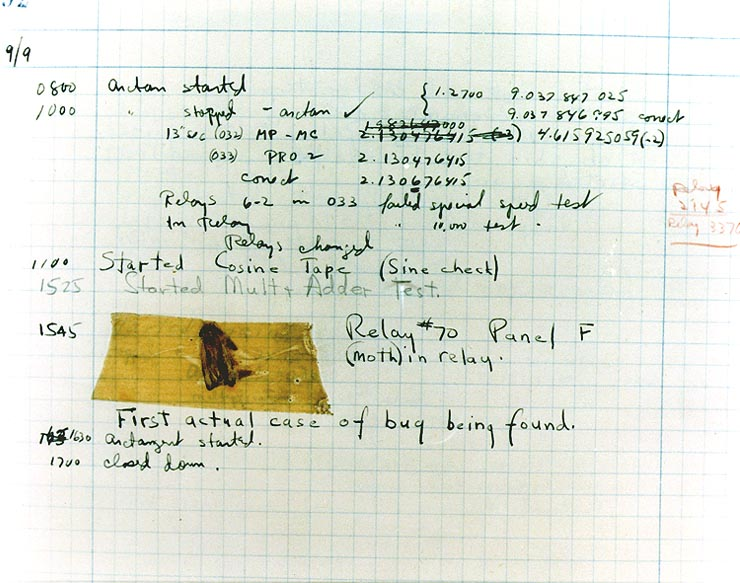
\includegraphics[width=0.6\textwidth]{first-bug.jpg}};
        \onslide<2->
        \node[anchor=south west, opacity=0.2] at (0,-36ex) {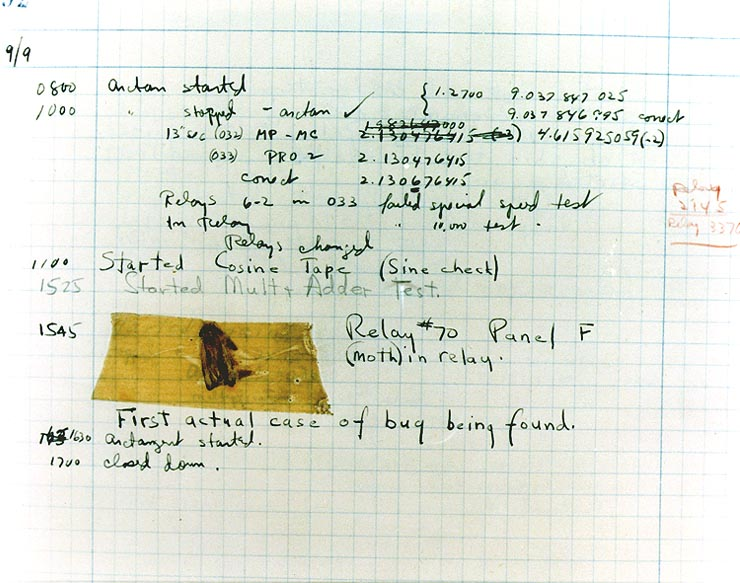
\includegraphics[width=0.6\textwidth]{first-bug.jpg}};
        \node[anchor=south west] at (0,-36ex) {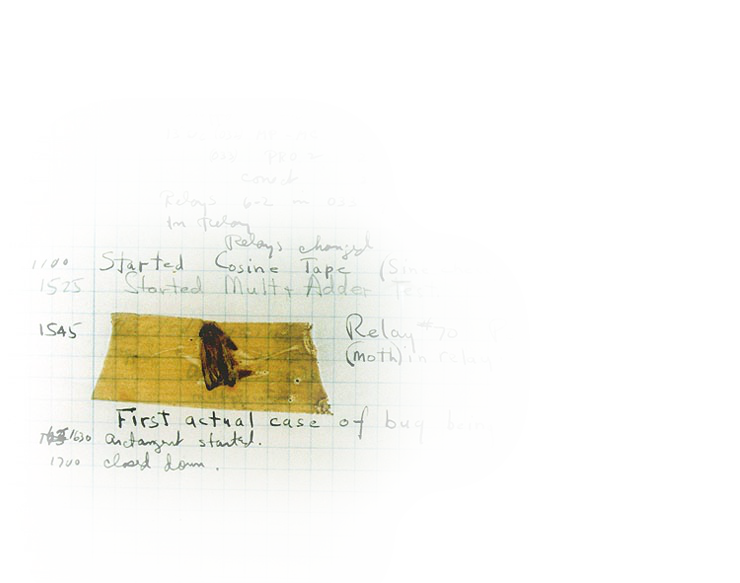
\includegraphics[width=0.6\textwidth]{first-bug.png}};
        \onslide<1->
    \end{tikzpicture}
    \pause  
    \tikz[overlay]\node[rotate=-6] at (60ex,10ex) {
\includegraphics[width=0.25\textwidth]{wikipedia.png}};
    In 1946, when \textbf{[Grace] Hopper} was released from active duty, she joined the Harvard Faculty at the Computation Laboratory where she continued her work on the Mark II and Mark III. Operators traced an error in the Mark II to a moth trapped in a relay, coining the term bug. This bug was carefully removed and taped to the log book. Stemming from the first bug, today we call errors or glitches in a program a bug.
\end{frame}

\begin{frame}
    \frametitle{Does it happen?}
    \tikz[overlay]\node[rotate=-6] at (60ex,9ex) {
\includegraphics[width=0.23\textwidth]{Stroustrup_PPP.jpg}};
    \begin{itemize}[<+->]
        \item When we write programs, errors are natural and unavoidable.
        \item \textit{The last bug} is a programmers’ joke.
        \item By the time we might have, we are busy modifying the program for some new use.
    \end{itemize}
\end{frame}

\begin{frame}
    \frametitle{Does it matter?}
    \begin{itemize}[<+->]
        \item Therac-25 Radiation Therapy Machine \small$\longrightarrow$ overdosed six people
        \item Northeast Blackout of 2003 \small$\longrightarrow$ 55,000,000 people affected 
        \item Pentium FDIV Bug \small$\longrightarrow$ \$475,000,000 cost
        \item NASA Mariner 1 Destruction \small$\longrightarrow$ \$18,500,000 cost
        \item Year 2000 Problem
    \end{itemize}
\end{frame}

\begin{frame}
    \frametitle{Why does it happen?}
    \tikz[overlay]\node[rotate=-6] at (60ex,4ex) {
\includegraphics[width=0.25\textwidth]{Stroustrup_PPP.jpg}};
    \begin{itemize}[<+->]
        \item poor specification
        \item incomplete programs
        \item unexpected inputs \& arguments
        \item unexpected state
        \item logical errors
    \end{itemize}
    \onslide<+->Errors are always more common when you are tired or rushed.
\end{frame}

\begin{frame}
    \frametitle{What should we do?}
    \begin{itemize}[<+->]
        \item debug
        \item test
        \item formal verification
        \item design for test \& debug\onslide<+->, write clean codes
    \end{itemize}
    {\onslide<3-3| handout:0>\tikz[overlay,anchor=west]\node at (0.4\textwidth,6ex) {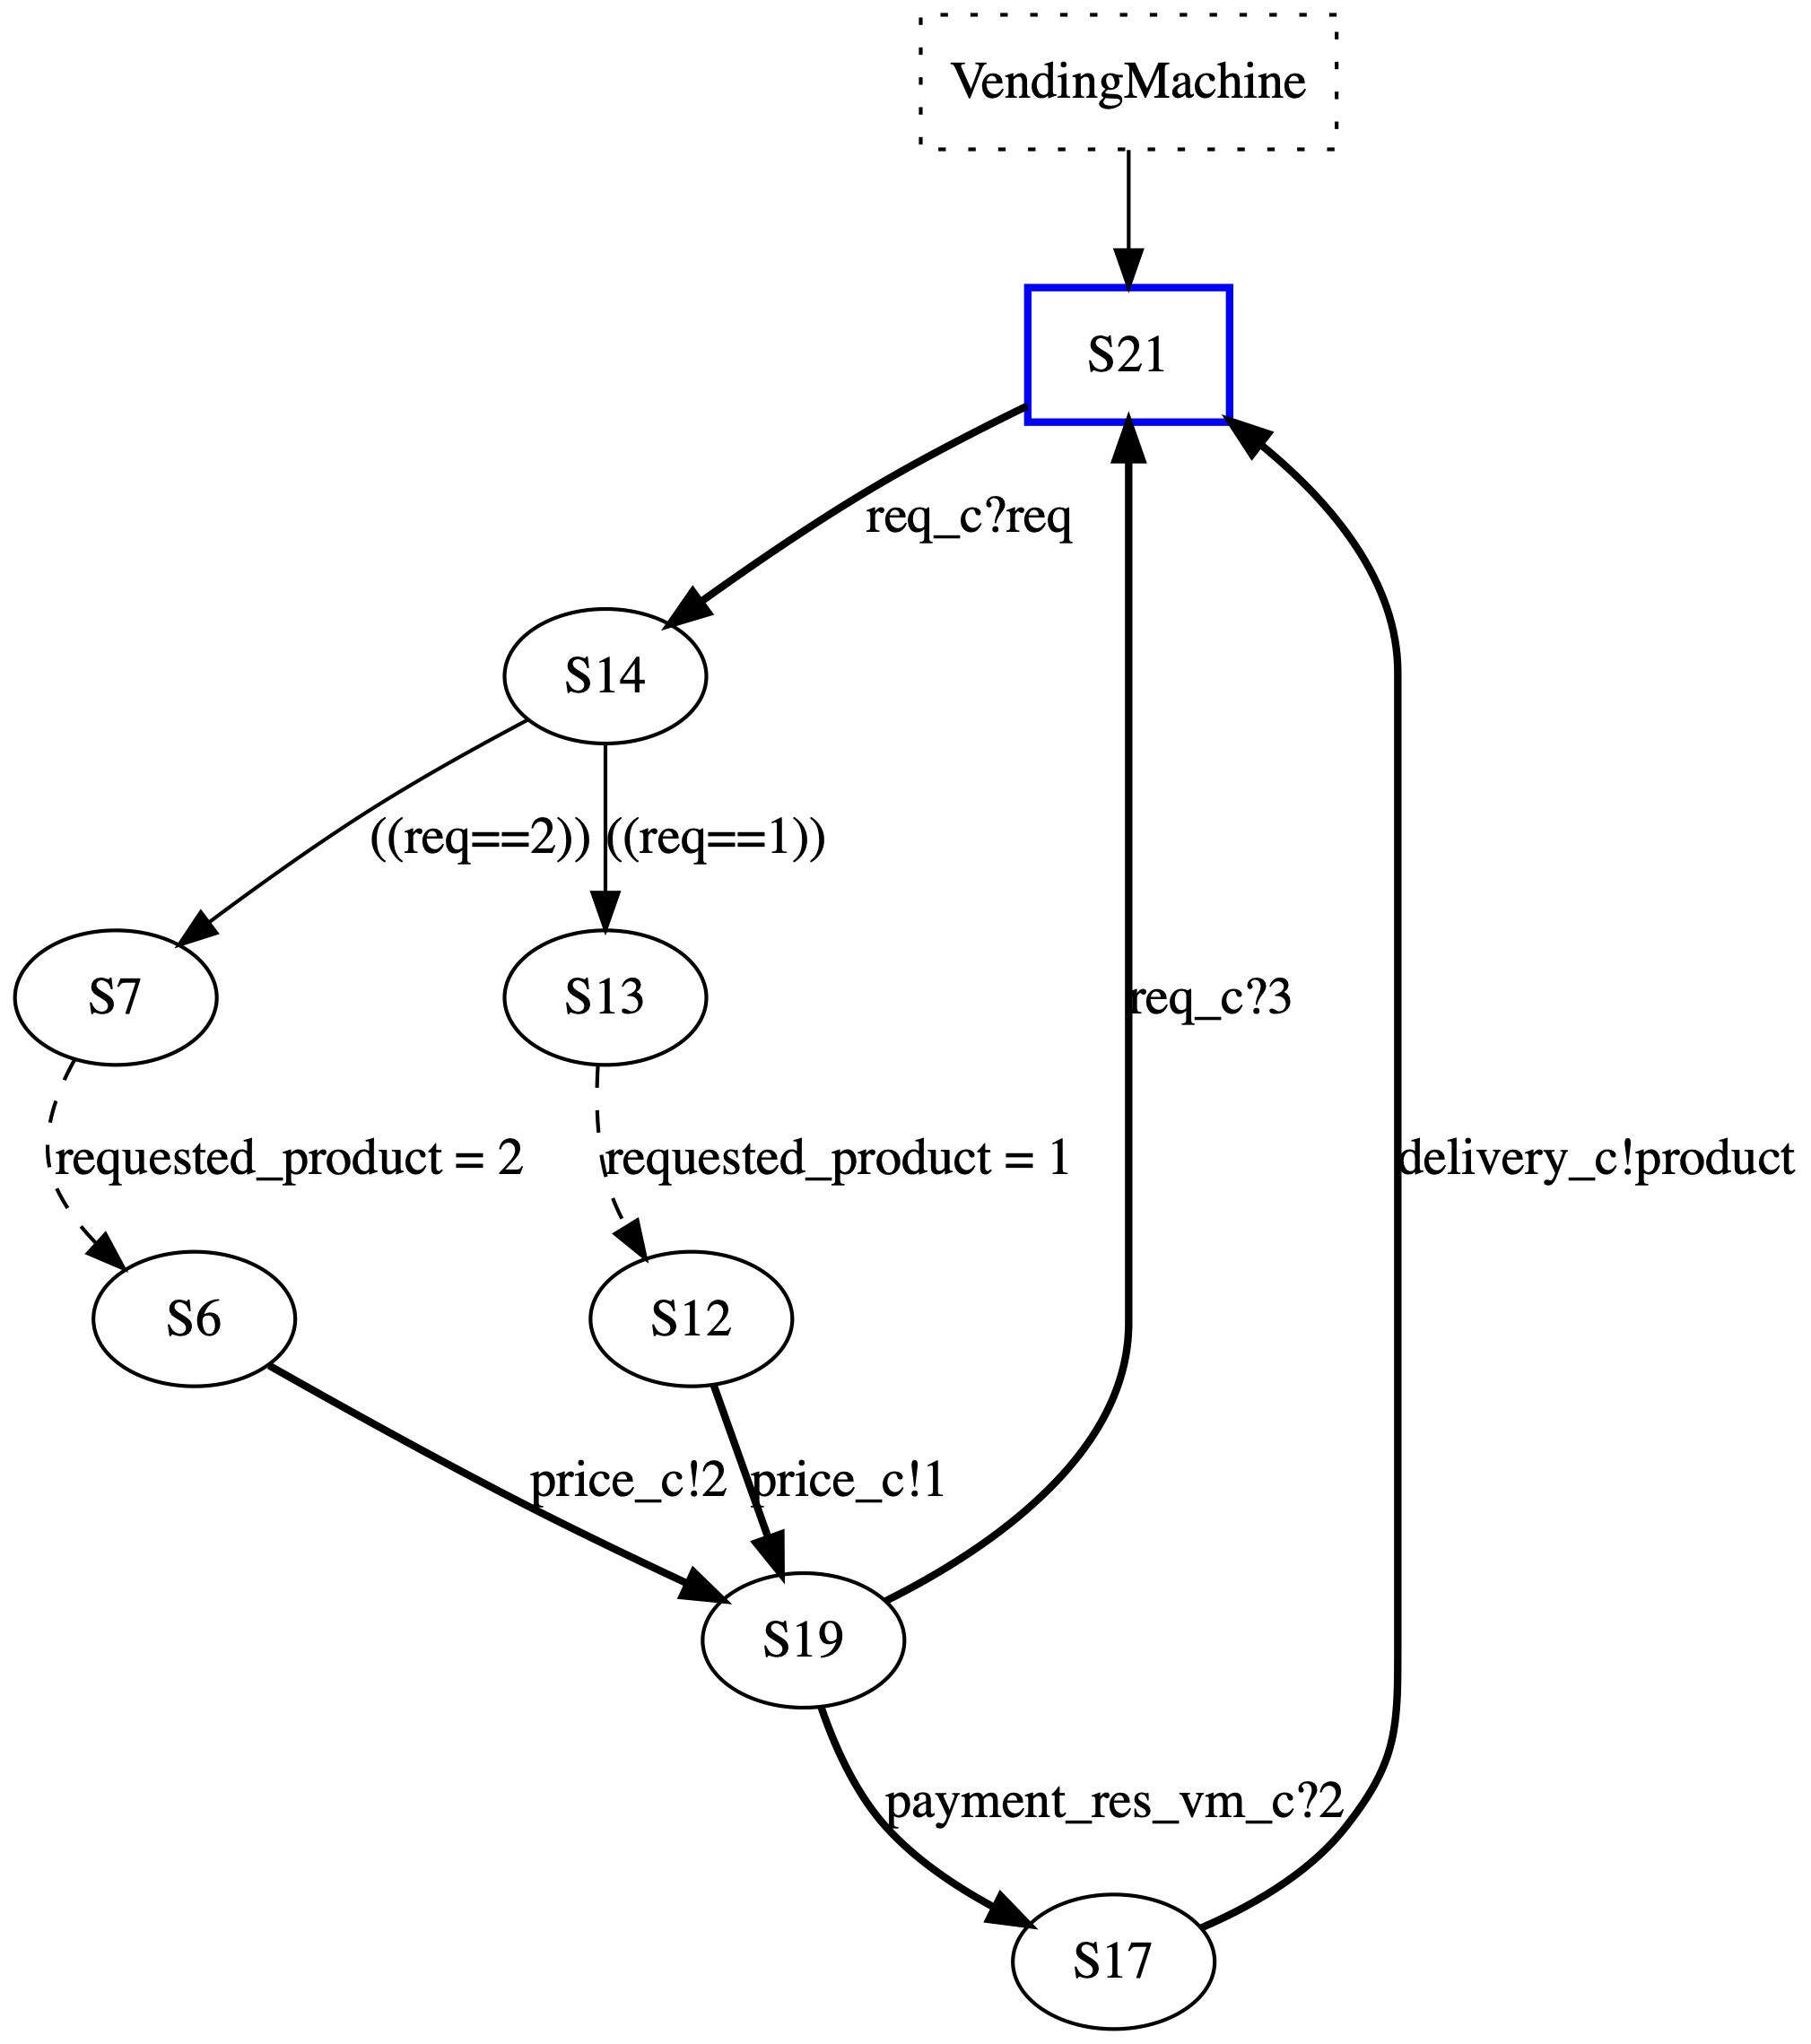
\includegraphics[height=0.8\textheight]{vm}};}
    {\onslide<2-2| handout:0>\tikz[overlay,anchor=west]\node at (0.2\textwidth,6ex) {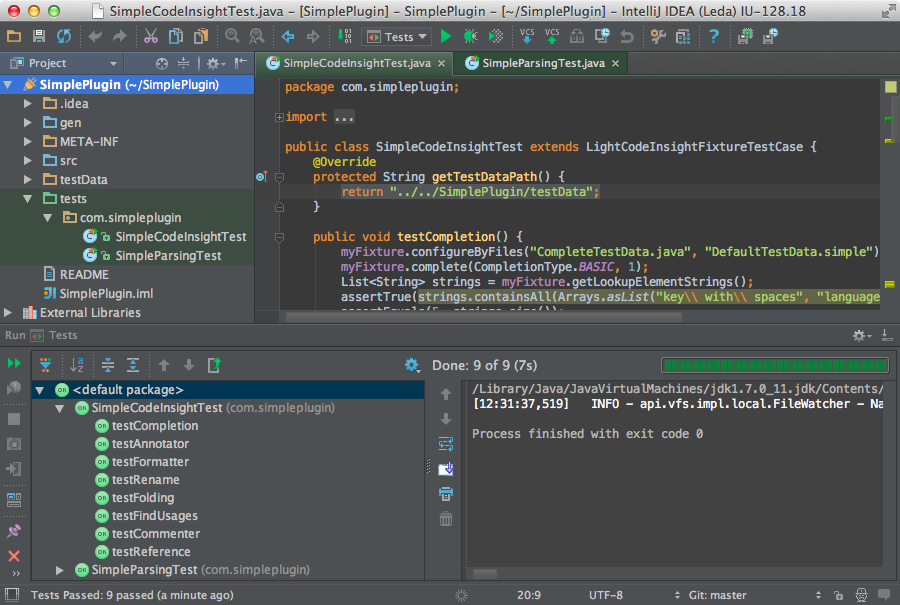
\includegraphics[width=0.7\textwidth]{plugin_tests_overview.png}};}
\end{frame}

\begin{frame}
    \frametitle{How far should we go?}
    \tikz[overlay]\node[rotate=-6] at (60ex,7ex) {
\includegraphics[width=0.25\textwidth]{Stroustrup_PPP.jpg}};
    \begin{itemize}[<+->]
        \item Eliminating \textit{all} errors?
        \item What about kicking out the power cord from the computer while it executed the program?
        \item What about data lose in safety-critical systems such as a medical monitoring program or the control program for a telephone switch?
    \end{itemize}
\end{frame}

\subsection{Debug}

\begin{frame}
    \frametitle{Debugging is hard}
    \begin{figure}
        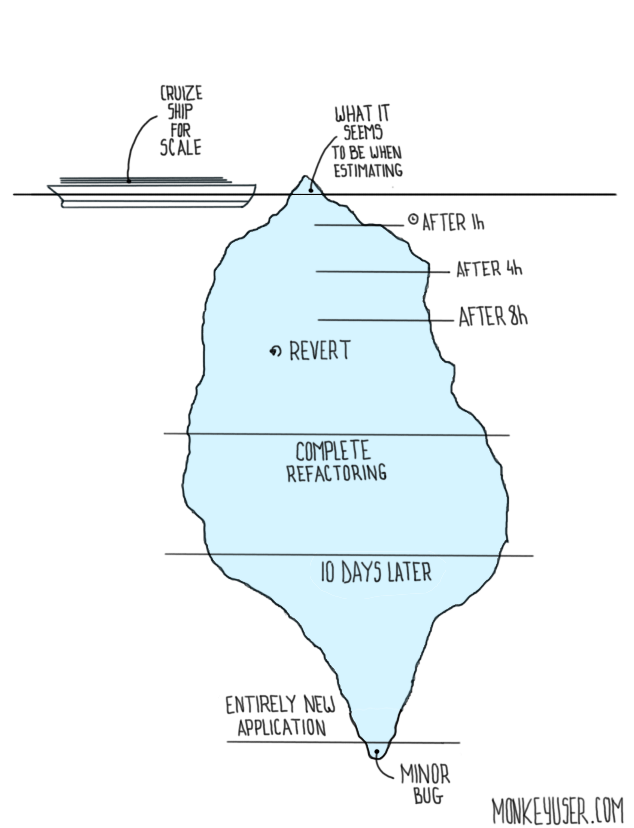
\includegraphics[height=0.8\textheight]{minor-bug.png}
    \end{figure}
\end{frame}

\begin{frame}
    \frametitle{Debugging is really hard}
    \begin{quote}
        Everyone knows that debugging is twice as hard as writing a program in the first place.

        \hfill\scriptsize ---~Brian Kernighan
    \end{quote}
\end{frame}

\begin{frame}
    \frametitle{Bugs are complex}
    \begin{figure}
        
\includegraphics[height=0.8\textheight]{root-cause.png}
    \end{figure}
\end{frame}

% !TeX root=debugging.tex

\section{Types of bugs}

\begin{frame}
    \frametitle{Types of bugs}
    \begin{figure}
        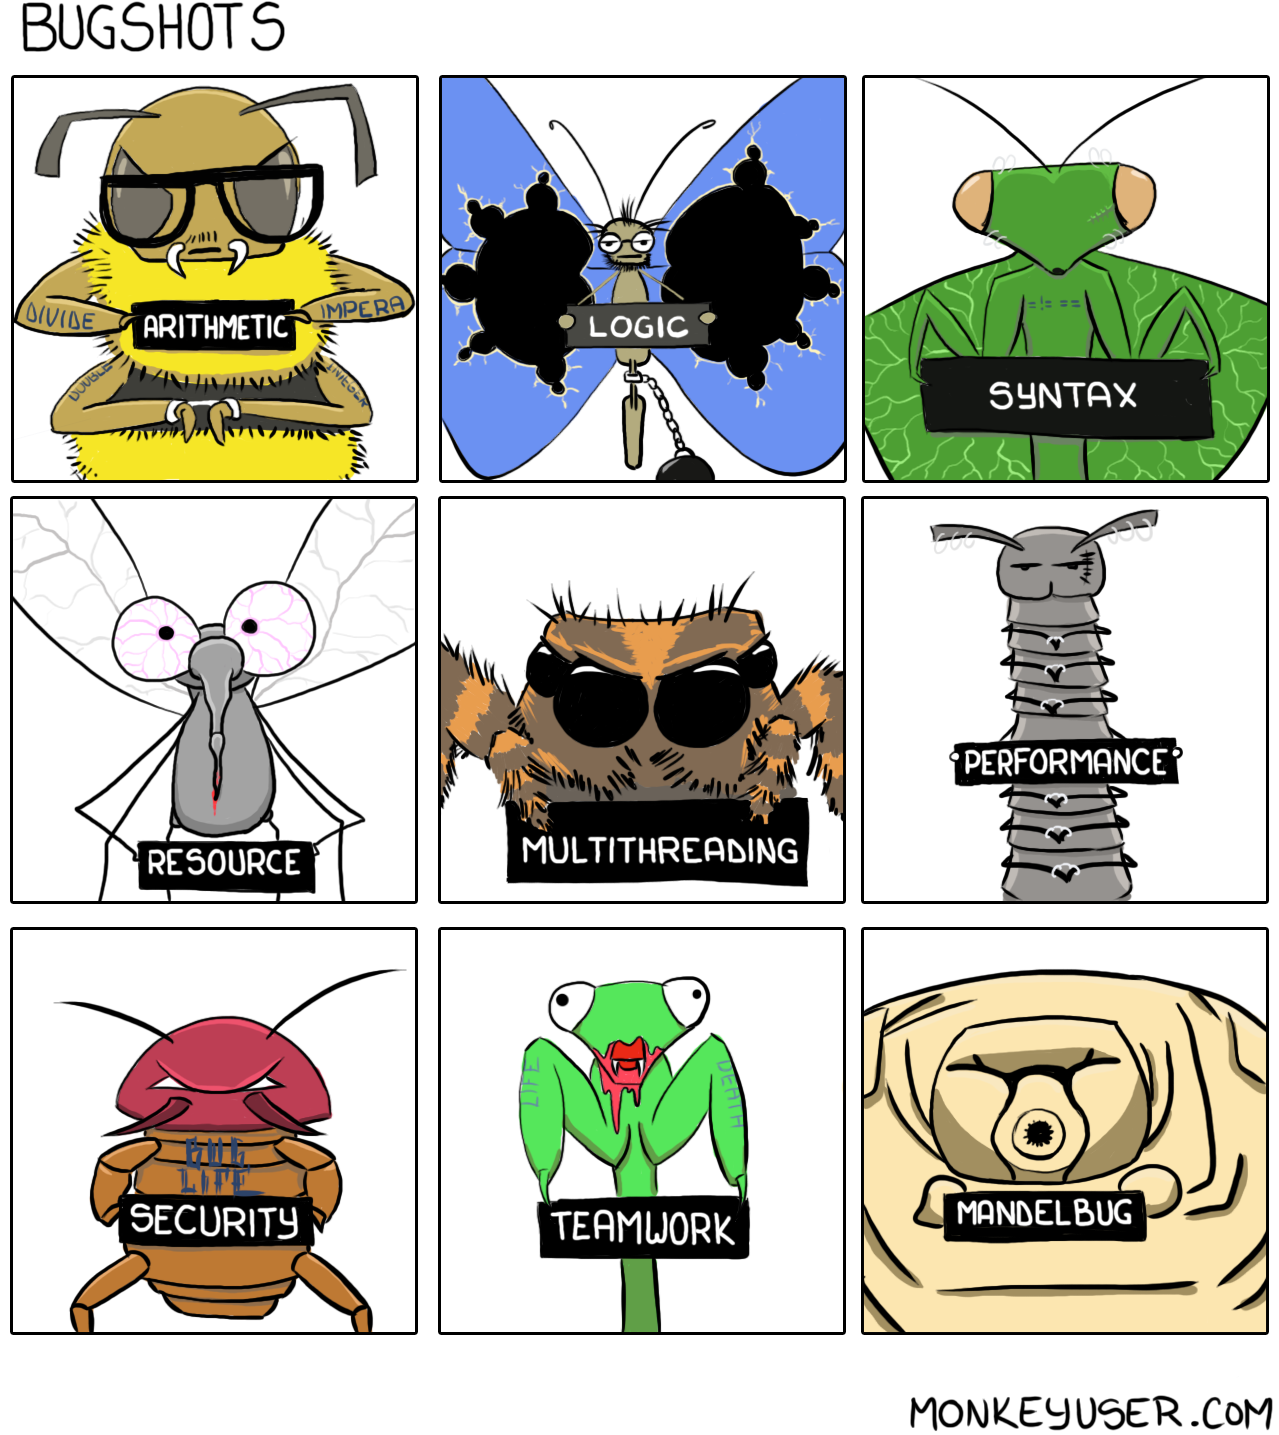
\includegraphics[height=0.8\textheight]{bugshots.png}
    \end{figure}
\end{frame}

\begin{frame}
    \frametitle{Types of bugs}
    \tikz[overlay]\node[rotate=-6] at (60ex,6ex) {
\includegraphics[width=0.3\textwidth]{Stroustrup_PPP.jpg}};
    \tikz[overlay]\node[rotate=-6] at (57ex,-9ex) {\footnotesize Chapter 5: Errors};
    \begin{itemize}[<+->]
        \item Compile-time errors
        \item Run-time errors
        \item Logic errors
    \end{itemize}
\end{frame}

\subsection<beamer:0>{Compile-time errors}

\begin{frame}<beamer:0>[fragile]
    \frametitle{Compile-time errors}
    \tikz[overlay]\node[rotate=-6] at (60ex,3ex) {
\includegraphics[width=0.23\textwidth]{Stroustrup_PPP.jpg}};
    \begin{itemize}[<+->]
        \item compiler-time errors
        \begin{itemize}[<+->]
            \item syntax errors
            \item type errors
            \item non-errors\onslide<+-> \qquad$\longrightarrow$ As you gain experience, you’ll begin to wish that the compiler would reject more code, rather than less.
            \begin{lstlisting}[]
int area(int length, int width); // calculate area of a rectangle

int x = area(10, -7); // OK: but a rectangle with a negative width?
int y = area(10.7, 9.3); // OK: but calls area(10, 9)
char z = area(100, 9999); // OK: but truncates the result
            \end{lstlisting}
        \end{itemize}
        \item link-time errors
    \end{itemize}
\end{frame}

\begin{frame}
    \frametitle{C++ build process}
    \begin{figure}
        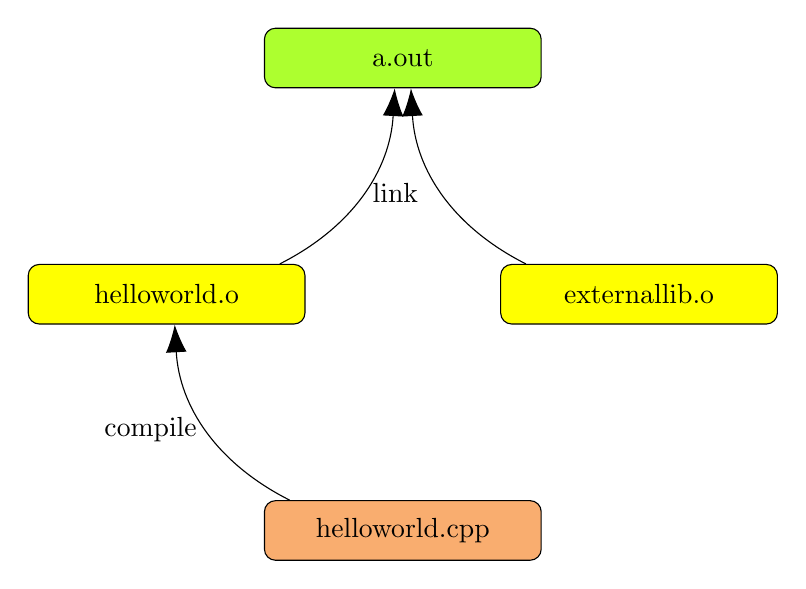
\begin{tikzpicture}
            \node[rectangle, draw, minimum width=10em, minimum height=5ex, rounded corners, fill=Apricot] (hwcpp) at (3,0) {helloworld.cpp};
            \node[rectangle, draw, minimum width=10em, minimum height=5ex, rounded corners, fill=Yellow] (hwobj) at (0,3) {helloworld.o};
            \node[rectangle, draw, minimum width=10em, minimum height=5ex, rounded corners, fill=Yellow] (libobj) at (6,3) {externallib.o};
            \node[rectangle, draw, minimum width=10em, minimum height=5ex, rounded corners, fill=GreenYellow] (exec) at (3,6) {a.out};
            \draw[-{Latex[length=1em]}, bend left] (hwcpp) to node[midway, left] {compile} (hwobj);
            \draw[-{Latex[length=1em]}, bend right] (hwobj) to node[midway, right] {link} (exec);
            \draw[-{Latex[length=1em]}, bend left] (libobj) to (exec);
        \end{tikzpicture}
    \end{figure}
\end{frame}

\subsection<beamer:0>{Run-time errors}

\begin{frame}<beamer:0>
    \frametitle{Run-time errors}
    \tikz[overlay]\node[rotate=-6] at (60ex,5ex) {
\includegraphics[width=0.23\textwidth]{Stroustrup_PPP.jpg}};
    \begin{itemize}[<+->]
        \item run-time errors
        \begin{itemize}[<+->]
            \item integration errors
            \item error reporting
            \item range errors
            \item bad inputs
            \item narrowing errors
            \item memory access errors
        \end{itemize}
    \end{itemize}
\end{frame}

\begin{frame}<beamer:0>
    \frametitle{Integration errors}
    \tikz[overlay]\node[rotate=-6] at (60ex,0ex) {
\includegraphics[width=0.23\textwidth]{Stroustrup_PPP.jpg}};
    Who should deal with errors in function calls?
    \onslide<+->
    \begin{itemize}[<+->]
        \item caller
            \begin{itemize}[<+->]
                \item code duplication
                \item are all calls error-checked?
            \end{itemize}
        \item callee
            \begin{itemize}[<+->]
                \item we can’t modify the function definition (e.g. library functions)
                \item it doesn’t know what to do in case of error
                \item it doesn’t know where it was called from
                \item performance
            \end{itemize}
    \end{itemize}
    \onslide<+->So\dots\\
    \onslide<+->Check your arguments in a function unless you have a good reason not to.
\end{frame}

\begin{frame}<beamer:0>
    \frametitle{Error reporting}
    \begin{itemize}[<+->]
        \item \texttt{cerr} \& \texttt{stderr} \onslide<+-> $\longrightarrow$ redirection: \texttt{./a.out 2> err.txt}
        \item return value
        \begin{itemize}[<+->]
            \item special values
            \item \texttt{read}, \texttt{write}, \texttt{listen} (\texttt{-1}, in combination with \texttt{errno})
            \item C++ \texttt{main} function \onslide<+-> $\longrightarrow$ \texttt{0}\onslide<+->, \texttt{cstdlib} \texttt{EXIT\_SUCCESS} \& \texttt{EXIT\_FAILURE}
            \item \texttt{exit()} (\texttt{cstdlib})
        \end{itemize}
        \item flag
        \begin{itemize}[<+->]
            \item \texttt{errno} (\texttt{errno.h})\onslide<+->, \texttt{perror} (\texttt{stdio.h})\onslide<+->, \texttt{strerror} (\texttt{string.h})
            \item \texttt{stream} error state flags\onslide<+->: \texttt{good()}\onslide<+->, \texttt{eof()}\onslide<+->, \texttt{fail()}\onslide<+->, \texttt{bad()}
        \end{itemize}
        \item exceptions
        \begin{itemize}[<+->]
            \item \texttt{throw} \& \texttt{catch}
            \item whoever could handle the error should catch the exception
            \item rethrow\onslide<+->: open files\onslide<+->, dynamically allocated memory cells
            \item \texttt{cstdexcept}
            \item not to throw exception in destructors
            \item inheritance \& subtyping
        \end{itemize}
    \end{itemize}
\end{frame}

\subsection<beamer:0>{Logic errors}

\begin{frame}<beamer:0>
    \frametitle{Logic errors}
    \tikz[overlay]\node[rotate=-6] at (60ex,4ex) {
\includegraphics[width=0.23\textwidth]{Stroustrup_PPP.jpg}};
    \begin{itemize}[<+->]
        \item the most difficult to find and eliminate
        \item sources:
        \begin{itemize}[<+->]
            \item your understanding of the underlying program logic is flawed
            \item you didn’t write what you thought you wrote
            \item you made some silly error
        \end{itemize}
        \item estimation
        \begin{itemize}[<+->]
            \item Is this answer to this particular problem plausible?
            \item How would I recognize a plausible result?
        \end{itemize}
    \end{itemize}
\end{frame}


\section{How to debug}
% !TeX root=debugging.tex

\subsection{Approaches}

\begin{frame}
    \frametitle{False assumptions}
    \tikz[overlay]\node[anchor=east] at (70ex,8ex) {\tiny\href{https://sway.office.com/PavDhCql8Adms1Ap}{\textit{The Art of Debugging}}, Ehsan Hajyasini, UT AP F96};
    Finding your bug is a process of confirming the many things you believe are true, until you find one which is not true.
    \onslide<+->
    \begin{itemize}[<+->]
        \item you believe that at a certain point in your source file, a certain \textbf{variable} has a certain \textbf{value}
        \item you believe that in a given \texttt{if-then-else} statement, the \texttt{else} \textbf{branch} is the one that is \textbf{executed}
        \item you believe that when you call a certain function, the \textbf{function} \textbf{receives} its \textbf{parameters} correctly
    \end{itemize}
    \onslide<+->So\dots check the assumptions!\onslide<+-> $\longrightarrow$ binary search\onslide<+->, pre \& post conditions
\end{frame}

\begin{frame}
    \frametitle{Stabilize, isolate, minimize}
    \tikz[overlay]\node[anchor=east] at (70ex,14ex) {\tiny\href{https://sway.office.com/PavDhCql8Adms1Ap}{\textit{The Art of Debugging}}, Ehsan Hajyasini, UT AP F96};
    \begin{itemize}[<+->]
        \item make failure-inducing \textbf{input smaller} \onslide<+->$\longrightarrow$ is more relevant\onslide<+->, saves time
        \item make the program \textbf{crash faster}
        \item make the situation \textbf{deterministic} \onslide<+->$\longrightarrow$ make bugs \textbf{reproducible}
    \end{itemize}
\end{frame}

\begin{frame}
    \frametitle{Reproducing bugs}
    \begin{figure}
        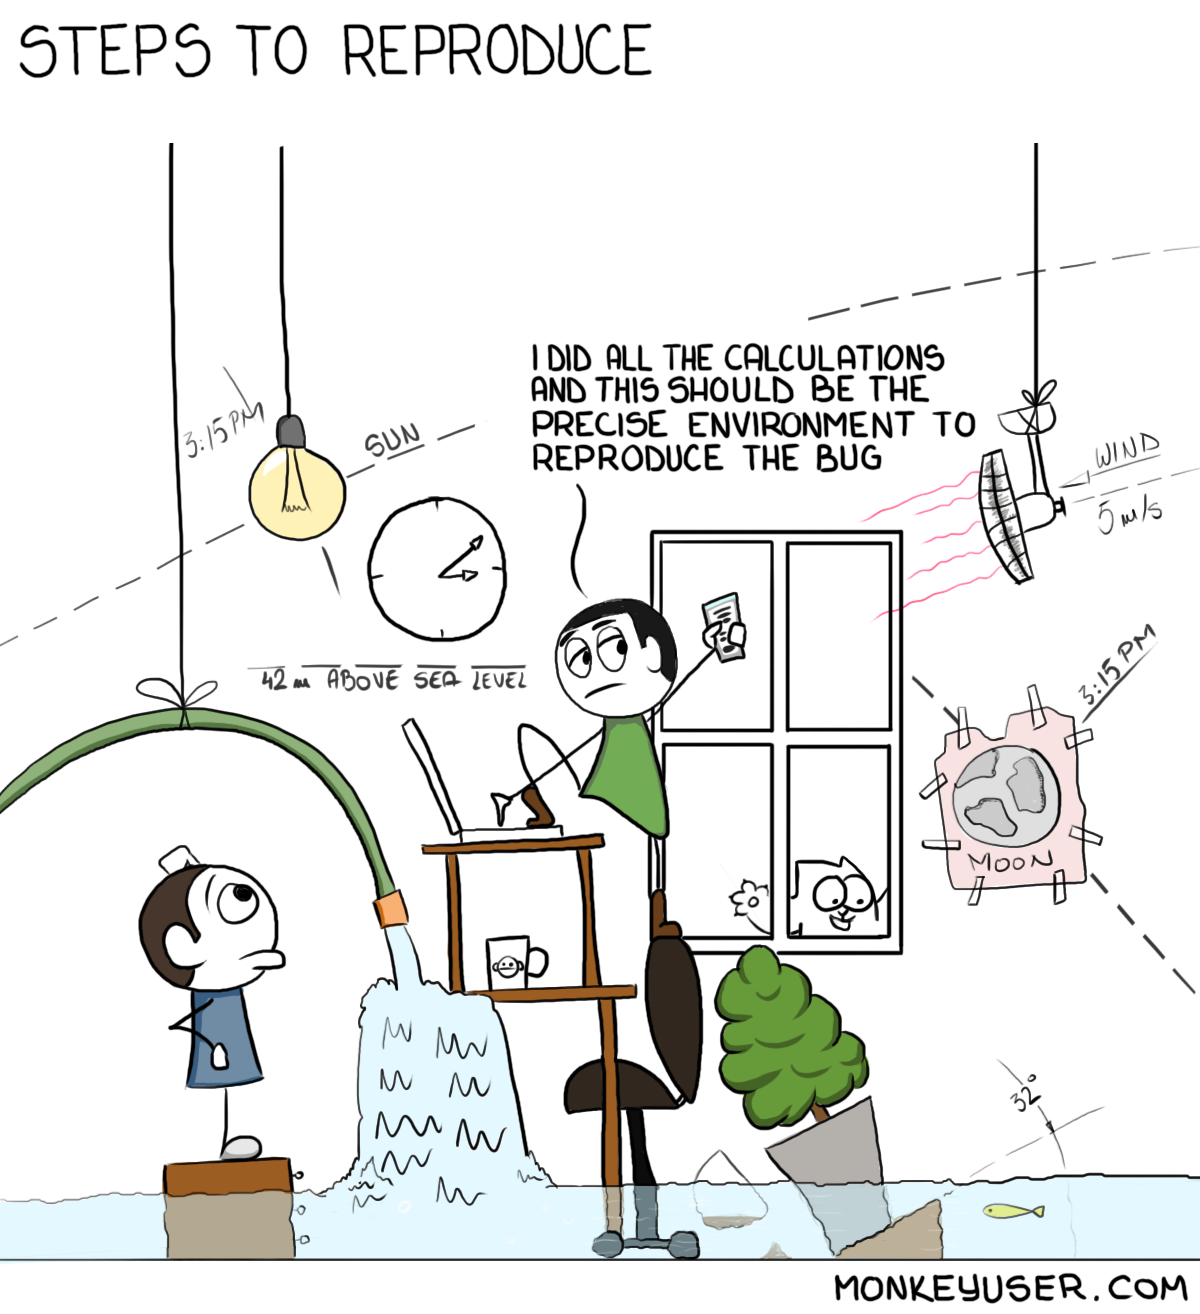
\includegraphics[height=0.8\textheight]{steps-to-reproduce.png}
    \end{figure}
\end{frame}

\begin{frame}
    \frametitle{Scientific method of debugging}
    \tikz[overlay]\node[anchor=east] at (58ex,5ex) {\tiny\textit{Debugging}, Max Goldman and Rob Miller, \href{http://web.mit.edu/6.031/www/fa17/}{MIT Software Construction (6.031) F17}};
    \tikz[overlay]\node[rotate=-6] at (63ex,4.5ex) {
\includegraphics[width=0.13\textwidth]{whyprogramsfail.jpg}};
    \begin{enumerate}[<+->]
        \item \textbf{study the data} \onslide<+->$\longrightarrow$ incorrect results\onslide<+->, failed assertions\onslide<+->, stack traces
        \item \textbf{hypothesize} \onslide<+->$\longrightarrow$ where the bug might be\onslide<+->, or where it cannot be
            \begin{itemize}[<+->]
                \item \textbf{slicing} \onslide<+->$\longrightarrow$ When you have a failure the \textit{slice} for that value consists of the lines of the program that helped compute the bad value.
                \item \textbf{delta debugging} \onslide<+->$\longrightarrow$ difference between successful execution and failing execution\onslide<+->: test cases\onslide<+->, \href{https://martinfowler.com/bliki/DiffDebugging.html}{diff debugging} \& undoing changes 
                \item \textbf{swap components} \onslide<+->$\longrightarrow$ different implementations
            \end{itemize}
            \onslide<+->\textbf{prioritizing hypotheses} \onslide<+->$\longrightarrow$ old, well-tested code vs recently-added code\onslide<+->, library code vs your code
        \item \textbf{experiment} \onslide<+->$\longrightarrow$ devise and run an experiment 
        \item \textbf{repeat}
    \end{enumerate}
\end{frame}

\begin{frame}[fragile]
    \frametitle{Stack trace}
    \begin{Verbatim}[fontsize=\tiny]
Traceback (most recent call last):
  File "./__main__.py", line 154, in <module>
    main()
  File "./__main__.py", line 145, in main
    config = extract_config(config_file_addr)
  File "./__main__.py", line 21, in extract_config
    config = DictWrapper(json.load(f))
  File "/usr/local/Cellar/python/.../3.7/lib/python3.7/json/__init__.py", line 296, in load
    parse_constant=parse_constant, object_pairs_hook=object_pairs_hook, **kw)
  File "/usr/local/Cellar/python/.../3.7/lib/python3.7/json/__init__.py", line 348, in loads
    return _default_decoder.decode(s)
  File "/usr/local/Cellar/python/.../3.7/lib/python3.7/json/decoder.py", line 337, in decode
    obj, end = self.raw_decode(s, idx=_w(s, 0).end())
  File "/usr/local/Cellar/python/.../3.7/lib/python3.7/json/decoder.py", line 353, in raw_decode
    obj, end = self.scan_once(s, idx)
json.decoder.JSONDecodeError: Expecting property name enclosed in double quotes: line 43 column 5 (char 1114)
    \end{Verbatim}
\end{frame}

% !TeX root=debugging.tex

\subsection{Tools}

\begin{frame}
    \frametitle{Compiler logs}
    \begin{itemize}[<+->]
        \item compiler errors
        \begin{itemize}[<+->]
            \item compiler errors
            \item link errors \onslide<+-> $\longrightarrow$ harder to read
        \end{itemize}
        \item start from the first one
        \item not always at the exact position
        \item language \& compiler version\onslide<+->: incompatibility\onslide<+->, better logs
        \item LLVM \& \texttt{clang++}
        \item compiler warnings
    \end{itemize}
\end{frame}

\begin{frame}[fragile]
    \frametitle{Stack trace}
    \begin{Verbatim}[fontsize=\tiny]
Traceback (most recent call last):
  File "./__main__.py", line 154, in <module>
    main()
  File "./__main__.py", line 145, in main
    config = extract_config(config_file_addr)
  File "./__main__.py", line 21, in extract_config
    config = DictWrapper(json.load(f))
  File "/usr/local/Cellar/python/.../3.7/lib/python3.7/json/__init__.py", line 296, in load
    parse_constant=parse_constant, object_pairs_hook=object_pairs_hook, **kw)
  File "/usr/local/Cellar/python/.../3.7/lib/python3.7/json/__init__.py", line 348, in loads
    return _default_decoder.decode(s)
  File "/usr/local/Cellar/python/.../3.7/lib/python3.7/json/decoder.py", line 337, in decode
    obj, end = self.raw_decode(s, idx=_w(s, 0).end())
  File "/usr/local/Cellar/python/.../3.7/lib/python3.7/json/decoder.py", line 353, in raw_decode
    obj, end = self.scan_once(s, idx)
json.decoder.JSONDecodeError: Expecting property name enclosed in double quotes: line 43 column 5 (char 1114)
    \end{Verbatim}
\end{frame}

\begin{frame}
    \frametitle{Compiler flags}
    \begin{itemize}[<+->]
        \item warning options
        \begin{description}[<+->]\footnotesize
            \item[\texttt{-Wall}] enable all the warnings about constructions that some users consider questionable
            \item[\texttt{-Wextra}] enable some extra warning flags that are not enabled by \texttt{-Wall}
            \item[\texttt{-pedantic}] issue all the warnings demanded by strict ISO C and ISO C++
        \end{description}
        \item debugging options
        \begin{description}[<+->]\footnotesize
            \item[\texttt{-g}] produce debugging information in the operating system’s native format
            \item[\texttt{-ggdb}] produce debugging information for use by GDB
        \end{description}
        \item sanitizers \footnotesize (\texttt{-fsanitize=})
        \begin{description}[<+->]\footnotesize
            \item[\texttt{address}] enable AddressSanitizer memory error detector
            \item[\texttt{leak}] enable LeakSanitizer memory leak detector
            \item[\texttt{undefined}] enable UndefinedBehaviorSanitizer undefined behaviour detector
        \end{description}
    \end{itemize}
\end{frame}

\begin{frame}
    \frametitle{External tools}
    \begin{description}[<+->]
        \item[\texttt{gdb}] the GNU Project debugger
        \item[\texttt{lldb}] LLVM debugger
        \item[\texttt{ddd}] a graphical front-end for command-line debuggers
        \item[\texttt{valgrind}] a programming tool for memory debugging, memory leak detection, and profiling
    \end{description}
\end{frame}


% \appendix

\end{document}
